
\subsection{Seasonal Temperature Trends}

Figures\ref{fig:Pre_monsoon_temperature_trends, fig:Monsoon_temperature_trends, fig:Post_monsoon_temperature_trends, fig:Winter_temperature_trends, fig:Annual_temperature_trends}  display temperature trend analyses based on three primary factors: temperature categories (Tavg, Tmax, Tmin), geographic regions (Himalayas, High Mountain, Middle Mountain, Siwalik, Tarai, and the entire Koshi Basin), and seasonal classifications (Monsoon, Post-monsoon, Pre-monsoon, Winter, and annual trends) across various decades. The trends reveal substantial variability influenced by decade, temperature type, physiographic region, and seasonal attributes.

\subsection*{Pre-monsoon}

\begin{figure}[H] 
  \centering
  \includegraphics[width=0.9\textwidth]{images/simple_plots_Premonsoon_Trend.png}  
  \caption{Pre-monsoon temperature trends across the time intervals (a) 1962–1971, (b) 1972–1981, (c) 1982–1991, (d) 1992–2001, (e) 2002–2011, (f) 2012–2021, and (g) 1962–2022.} 
  \label{fig:Pre_monsoon_temperature_trends}  
\end{figure}

Pre-monsoon season reveals overall cooling trends in the 1962-1971 decade except in Himalaya regions, similar cooling trend from 1972 to 1981, and later decade experience a warming trend except maximum and average temperature shows cooling trend in 2012-2021 (Figure \ref{fig:Pre_monsoon_temperature_trends}) For the overall period from 1962 to 2022, only the Siwalik region demonstrates a cooling trend; all other regions display warming trends, particularly the Himalayan region, which shows a higher rate of warming at 0.02$^\circ$C/year.  

\subsection*{Monsoon}
During the Monsoon season (Figure \ref{fig:Monsoon_temperature_trends}), temperature fluctuations have accelerated in recent decades, particularly from 2012 to 2021, with significant warming observed in average and minimum temperatures, while maximum temperatures predominantly show a cooling trend. Overall, from 1962 to 2022, the Monsoon season reflects a cooling trend across the various regions.

\begin{figure}[H] 
  \centering
  \includegraphics[width=0.9\textwidth]{images/simple_plots_Monsoon_Trend.png}  
  \caption{Monsoon temperature trends across the time intervals (a) 1962–1971, (b) 1972–1981, (c) 1982–1991, (d) 1992–2001, (e) 2002–2011, (f) 2012–2021, and (g) 1962–2022.} 
  \label{fig:Monsoon_temperature_trends}  
\end{figure}

\subsection*{Post-monsoon}

\begin{figure}[H] 
  \centering
  \includegraphics[width=0.9\textwidth]{images/simple_plots_Postmonsoon_Trend.png}
  \caption{Post-monsoon temperature trends across the time intervals (a) 1962–1971, (b) 1972–1981, (c) 1982–1991, (d) 1992–2001, (e) 2002–2011, (f) 2012–2021, and (g) 1962–2022.}
  \label{fig:Post_monsoon_temperature_trends}  
\end{figure}

A cooling trend is evident in the post-monsoon period from 1962 to 1981 (Figure \ref{fig:Post_monsoon_temperature_trends}), followed by a notable warming trend that has intensified in recent decades.

\subsection*{Winter}

\begin{figure}[H] 
  \centering
  \includegraphics[width=0.9\textwidth]{images/simple_plots_Winter_Trend.png}  
  \caption{Winter temperature trends across the time intervals (a) 1962–1971, (b) 1972–1981, (c) 1982–1991, (d) 1992–2001, (e) 2002–2011, (f) 2012–2021, and (g) 1962–2022.} 
  \label{fig:Winter_temperature_trends}  
\end{figure}


Distinct temperature trends are observed during the Winter season (Figure \ref{fig:Winter_temperature_trends}) across different regions and time periods. Minimum and average temperatures showed warming between 1982–1991 and 2012–2021, while a cooling trend occurred from 1962–1971. Maximum temperatures increased during the 1992–2001 and 2002–2011 decades, with a notable cooling of 0.52$^\circ$C in the High Mountain region from 2012 to 2021. Overall, from 1962 to 2022, the Siwalik region experienced a general cooling trend, while only the High Mountain region exhibited a warming trend.

\subsection*{Annual}

\begin{figure}[H] 
  \centering
  \includegraphics[width=0.9\textwidth]{images/simple_plots_annual_Trend.png}  
  \caption{Annual temperature trends across the time intervals (a) 1962–1971, (b) 1972–1981, (c) 1982–1991, (d) 1992–2001, (e) 2002–2011, (f) 2012–2021, and (g) 1962–2022.} 
  \label{fig:Annual_temperature_trends}  
\end{figure}

Figure \ref{fig:Annual temperature trends} illustrates the annual temperature trends across different regions of the Koshi Basin revealing significant variations over the decades. The first two decades (1962-1981) exhibit an overall cooling trend, with the exception of warming observed in the Himalayan regions, where maximum temperatures increased by 0.02 °C and minimum temperatures rose by 0.04 °C in later decades. The period from 1982 to 2021 predominantly shows a warming trend; however, from 2002 to 2011, the Siwalik region experienced a cooling trend, and in 2012 to 2021, maximum temperatures again exhibited a cooling trend. In overall annual temperature trends in Koshi Basin showed decreasing trend followed by increasing trend similar to study conducted by \textcite{chand_trend_2019} at Narayani Basin Nepal. 


Temporal and spatial analysis of five physiographic regions- Tarai, Siwalik, Middle-mountain, and High-mountain and Himalayas of Koshi Basin presented via Table \ref{tab:spatial_trends}.

\begin{table}[htbp]
  \centering
  \caption{Spatial distribution of temporal trends of temperature for 1962-2022}
  \begin{tabular}{@{}lcccccc@{}}
      \toprule
      Region & Tmax Trend & Tmax p-value & Tmin Trend & Tmin p-value & Tavg Trend & Tavg p-value \\ 
      \midrule
      \textbf{Himalaya} & & & & & & \\ 
      Monsoon & -0.0111 & 0.1672 & -0.0160 & 0.2340 & -0.0135 & 0.1964 \\ 
      Postmonsoon & 0.0114 & 0.1412 & -0.0011 & 0.9435 & 0.0051 & 0.6504 \\ 
      Premonsoon & \textbf{0.0186*} & 0.0115 & 0.0040 & 0.7977 & 0.0113 & 0.3058 \\ 
      Winter & 0.0031 & 0.7077 & -0.0177 & 0.0972 & -0.0073 & 0.4334 \\ 
      \midrule
      \textbf{High Mountain} & & & & & & \\ 
      Monsoon & -0.0038 & 0.5811 & \textbf{-0.023*} & 0.0019 & \textbf{-0.01*} & 0.0062 \\ 
      Postmonsoon & \textbf{0.0233*} & 0.0035 & 0.0128 & 0.1022 & \textbf{0.02*} & 0.0035 \\ 
      Premonsoon & 0.0125 & 0.0845 & \textbf{0.0164*} & 0.0103 & \textbf{0.01*} & 0.0084 \\ 
      Winter & \textbf{0.0317*} & 0.0058 & -0.0088 & 0.2583 & 0.0114 & 0.1407 \\ 
      \midrule
      \textbf{Middle Mountain} & & & & & & \\ 
      Monsoon & \textbf{-0.0122*} & 0.0338 & \textbf{-0.013*} & 0.0076 & \textbf{-0.01*} & 0.0157 \\ 
      Postmonsoon & 0.0032 & 0.5873 & 0.0011 & 0.8304 & 0.0021 & 0.6808 \\ 
      Premonsoon & 0.0071 & 0.2333 & 0.0074 & 0.1586 & 0.0072 & 0.1738 \\ 
      Winter & -0.0004 & 0.9422 & \textbf{-0.021*} & 0.0002 & \textbf{-0.01*} & 0.0466 \\ 
      \midrule
      \textbf{Siwalik} & & & & & & \\ 
      Monsoon & \textbf{-0.0552*} & 0.0000 & \textbf{-0.06*} & 0.0000 & \textbf{-0.06*} & 0.0000 \\ 
      Postmonsoon & -0.0135 & 0.0945 & \textbf{-0.04*} & 0.0000 & \textbf{-0.03*} & 0.0003 \\ 
      Premonsoon & -0.0106 & 0.1916 & \textbf{-0.04*} & 0.0005 & \textbf{-0.03*} & 0.0017 \\ 
      Winter & \textbf{-0.0260*} & 0.0030 & \textbf{-0.10*} & 0.0000 & \textbf{-0.06*} & 0.0000 \\ 
      \midrule
      \textbf{Tarai} & & & & & & \\ 
      Monsoon & \textbf{-0.0183*} & 0.0005 & -0.0215 & 0.0000 & -0.0199 & 0.0000 \\ 
      Postmonsoon & 0.0027 & 0.5809 & -0.0045 & 0.4620 & -0.0009 & 0.8552 \\ 
      Premonsoon & 0.0067 & 0.2577 & 0.0011 & 0.8275 & 0.0039 & 0.4280 \\ 
      Winter & -0.0006 & 0.9121 & -0.0280 & 0.0000 & -0.0143 & 0.0104 \\ 
      \bottomrule
  \end{tabular}
  \label{tab:spatial_trends}
  \begin{flushleft}
    \footnotesize{* Indicates \( p \leq 0.05 \) which denotes significant changes} \\
    
\end{flushleft}
\end{table}




In the five physiographic regions of Koshi Basin, temperature trends display distinct seasonal variations across physiographic regions (Table \ref{tab:spatial_trends}).

In the Himalaya region, a significant warming trend is observed during the pre-monsoon season in Tmax (0.0186, p=0.0115), while other trends remain largely non-significant, including slight cooling in the monsoon (Tmax: -0.0111, p=0.1672; Tmin: -0.0160, p=0.2340) and winter seasons (Tmin: -0.0177, p=0.0972).
The High Mountain region exhibits significant temperature changes across multiple seasons. In the post-monsoon, Tmax and Tavg show strong warming trends (Tmax: 0.0233, p=0.0035; Tavg: 0.0200, p=0.0035), while the monsoon season shows a significant cooling trend in Tmin (-0.0230, p=0.0019). The pre-monsoon season also reflects a notable warming in Tmin (0.0164, p=0.0103) and Tavg (0.0100, p=0.0084), with additional warming in Tmax during winter (0.0317, p=0.0058).
In the Middle Mountain region, a significant cooling trend is observed in the monsoon for both Tmax (-0.0122, p=0.0338) and Tmin (-0.0130, p=0.0076). The winter season also displays significant cooling in Tmin (-0.0210, p=0.0002) and Tavg (-0.0100, p=0.0466), while other seasons show minimal changes.
The Siwalik region experiences substantial cooling across all seasons, particularly in the monsoon, where strong cooling trends are present in Tmax (-0.0552, p=0.0000), Tmin (-0.0600, p=0.0000), and Tavg (-0.0600, p=0.0000). Similarly, significant cooling trends persist in the winter season (Tmax: -0.0260, p=0.0030; Tmin: -0.1000, p=0.0000; Tavg: -0.0600, p=0.0000).
In the Tarai region, notable cooling is observed during the monsoon in Tmax (-0.0183, p=0.0005), Tmin (-0.0215, p=0.0000), and Tavg (-0.0199, p=0.0000). Additionally, the winter season shows a marked cooling trend in Tmin (-0.0280, p=0.0000) and Tavg (-0.0143, p=0.0104), while other seasons display minimal trends.
Seasonal analysis reveals more diverse trends across regions. In the Hills and Middle Mountains, mixed patterns are evident, with significant declines in Tmin during the monsoon and winter seasons. In contrast, the High Mountains display minimal seasonal variation, aside from a notable increase in Tmax primarily during the pre-monsoon season. Significant seasonal cooling tendencies are visible in the Siwalik and Tarai areas, especially during the Monsoon and Winter, indicating different regional temperature behaviors. 

\textcite{shrestha_observed_2017} analyzed long-term trends in seasonal maximum and minimum temperatures from 1975 to 2010, finding widespread significant warming, particularly in minimum temperature indices, with stronger warming trends in recent decades; however, some stations showed declines in winter and pre-monsoon temperatures, and seasonal minimum temperatures generally increased more than maximum temperatures.

The study conducted by~\textcite{shrestha_climate_2011} identified consistent warming trends in seasonal mean maximum temperatures across all regions of Nepal from 1977 to 1994. Their study observed warming during the winter, post-monsoon, pre-monsoon, and monsoon seasons.
Study  by~\textcite{nayava_spatial_2017} for 1981–2010 showed varying seasonal temperature trends across Nepal. There is warming in the Terai, Valley, Hill and Mountain regions across all seasons from 0.01-0.13°C/year, with the Trans-Himalaya showing 0.03°C in pre-monsoon, -0.02°C in post-monsoon, 0.01°C in monsoon, and 0.08°C in winter. Similarly, \textcite{shrestha_maximum_1999}  showed significant regional and seasonal variations for 1977 to 1994 in temperature trends across Nepal, with the Trans-Himalaya experiencing the highest winter warming at 0.124°C/year, the Middle Mountains seeing the largest monsoon increase at 0.094°C/year, and the post-monsoon season showing an overall national average warming rate of 0.059°C/year, while the Terai region exhibited a much lower warming rate of 0.006°C/year in winter and -0.004°C/year in pre-monsoon.

\subsection{Regional Temperature Trends}

\begin{table}[htbp]
  \centering
  \caption{Regional temperature regression equations}
  \begin{tabular}{@{}lccc@{}}
      \toprule
      \textbf{Region} & \textbf{Tmin Equation} & \textbf{Tmax Equation} & \textbf{Tavg Equation} \\ 
      \midrule
      Himalaya & \( y = -0.01x + 15.46 \) & \( y = 0.00x + 2.58 \) & \( y = -0.00x + 9.02 \) \\ 
      High Mountain & \( y = -0.00x + 13.97 \) & \( y = 0.01x - 9.35 \) & \( y = 0.00x + 2.31 \) \\ 
      Middle Mountain & \( y = -0.01x + 27.88 \) & \( y = -0.00x + 27.81 \) & \( y = -0.00x + 27.85 \) \\ 
      Siwalik & \( y = -0.06x + 145.24 \) & \( y = -0.03x + 91.55 \) & \( y = -0.05x + 118.40 \) \\ 
      Tarai & \( y = -0.01x + 50.79 \) & \( y = -0.00x + 41.15 \) & \( y = -0.01x + 45.97 \) \\ 
      \bottomrule
  \end{tabular}
  \label{tab:regression_equations}
\end{table}


\begin{table}[H]
  \centering
  \caption{Nonparametric (Mann-Kendall Test) tests for annual regional trends for the period 1962–2022}
  \begin{tabular}{@{}lccc@{}}
      \toprule
      \textbf{Regions} & \textbf{Tmin Slope} & \textbf{Tmax Slope} & \textbf{Tavg Slope} \\ 
      \midrule
      Himalaya        & -0.009       & 0.005**      & -0.000** \\ 
      High Mountains  & -0.016       & 0.008**      & 0.002**  \\ 
      Middle Mountains & -0.008      & -0.001**     & -0.003** \\ 
      Siwalik         & -0.063       & -0.033       & -0.05    \\ 
      Tarai           & -0.015       & -0.003**     & -0.006** \\ 
      \bottomrule
  \end{tabular}
  \label{tab:mann_kendall}
  \begin{flushleft}
    \footnotesize{** indicates $p \geq 0.05$ which denotes no significant changes.}
\end{flushleft}
  \caption*{** indicates $p \geq 0.05$ which denotes no significant changes.}
\end{table}

The Annual Regional Mann-Kendall test findings are shown in the table 4. This test evaluates trends in minimum (Tmin), maximum (Tmax), and average (Tavg) temperatures in five regions: Tarai, Siwalik, Middle Mountains, High Mountains, and Himalaya. While Tmax and Tavg show rising tendencies (0.005** and -0.000**, respectively) in the Himalaya, the Tmin shows a decreasing trend (-0.009), and the latter two are not statistically significant (p $\geq$ 0.05). Tmin and Tavg (-0.008 and -0.003**) also exhibit declining patterns in the Middle-mountain, although Tmax (-0.001**) shows a rather constant trend. The High Mountains, on the other hand, show an increasing trend in Tmin (-0.016) and a more marked reduction in Tmax and Tavg (0.008** and 0.002**). All temperature measurements exhibit similar declines in the Siwalik region: Tmin (-0.063), Tmax (-0.033), and Tavg (-0.05). Lastly, with Tmin (-0.015), Tmax (-0.003**), and Tavg (-0.006**) showing diminishing trends across all temperature parameters; the Tarai likewise shows declining trends, but Tmax and Tavg are not statistically significant. In similar vein, the Koshi region's maximum temperature grew at a rate of 0.058 °C/year and its lowest temperature increased at a rate of 0.014 °C/year during the forty years leading up 1963 to 2009 \parencite{nepal_impacts_2016}.



\begin{figure}[htbp]
  \centering
  \begin{subfigure}{0.45\textwidth}
      \centering
      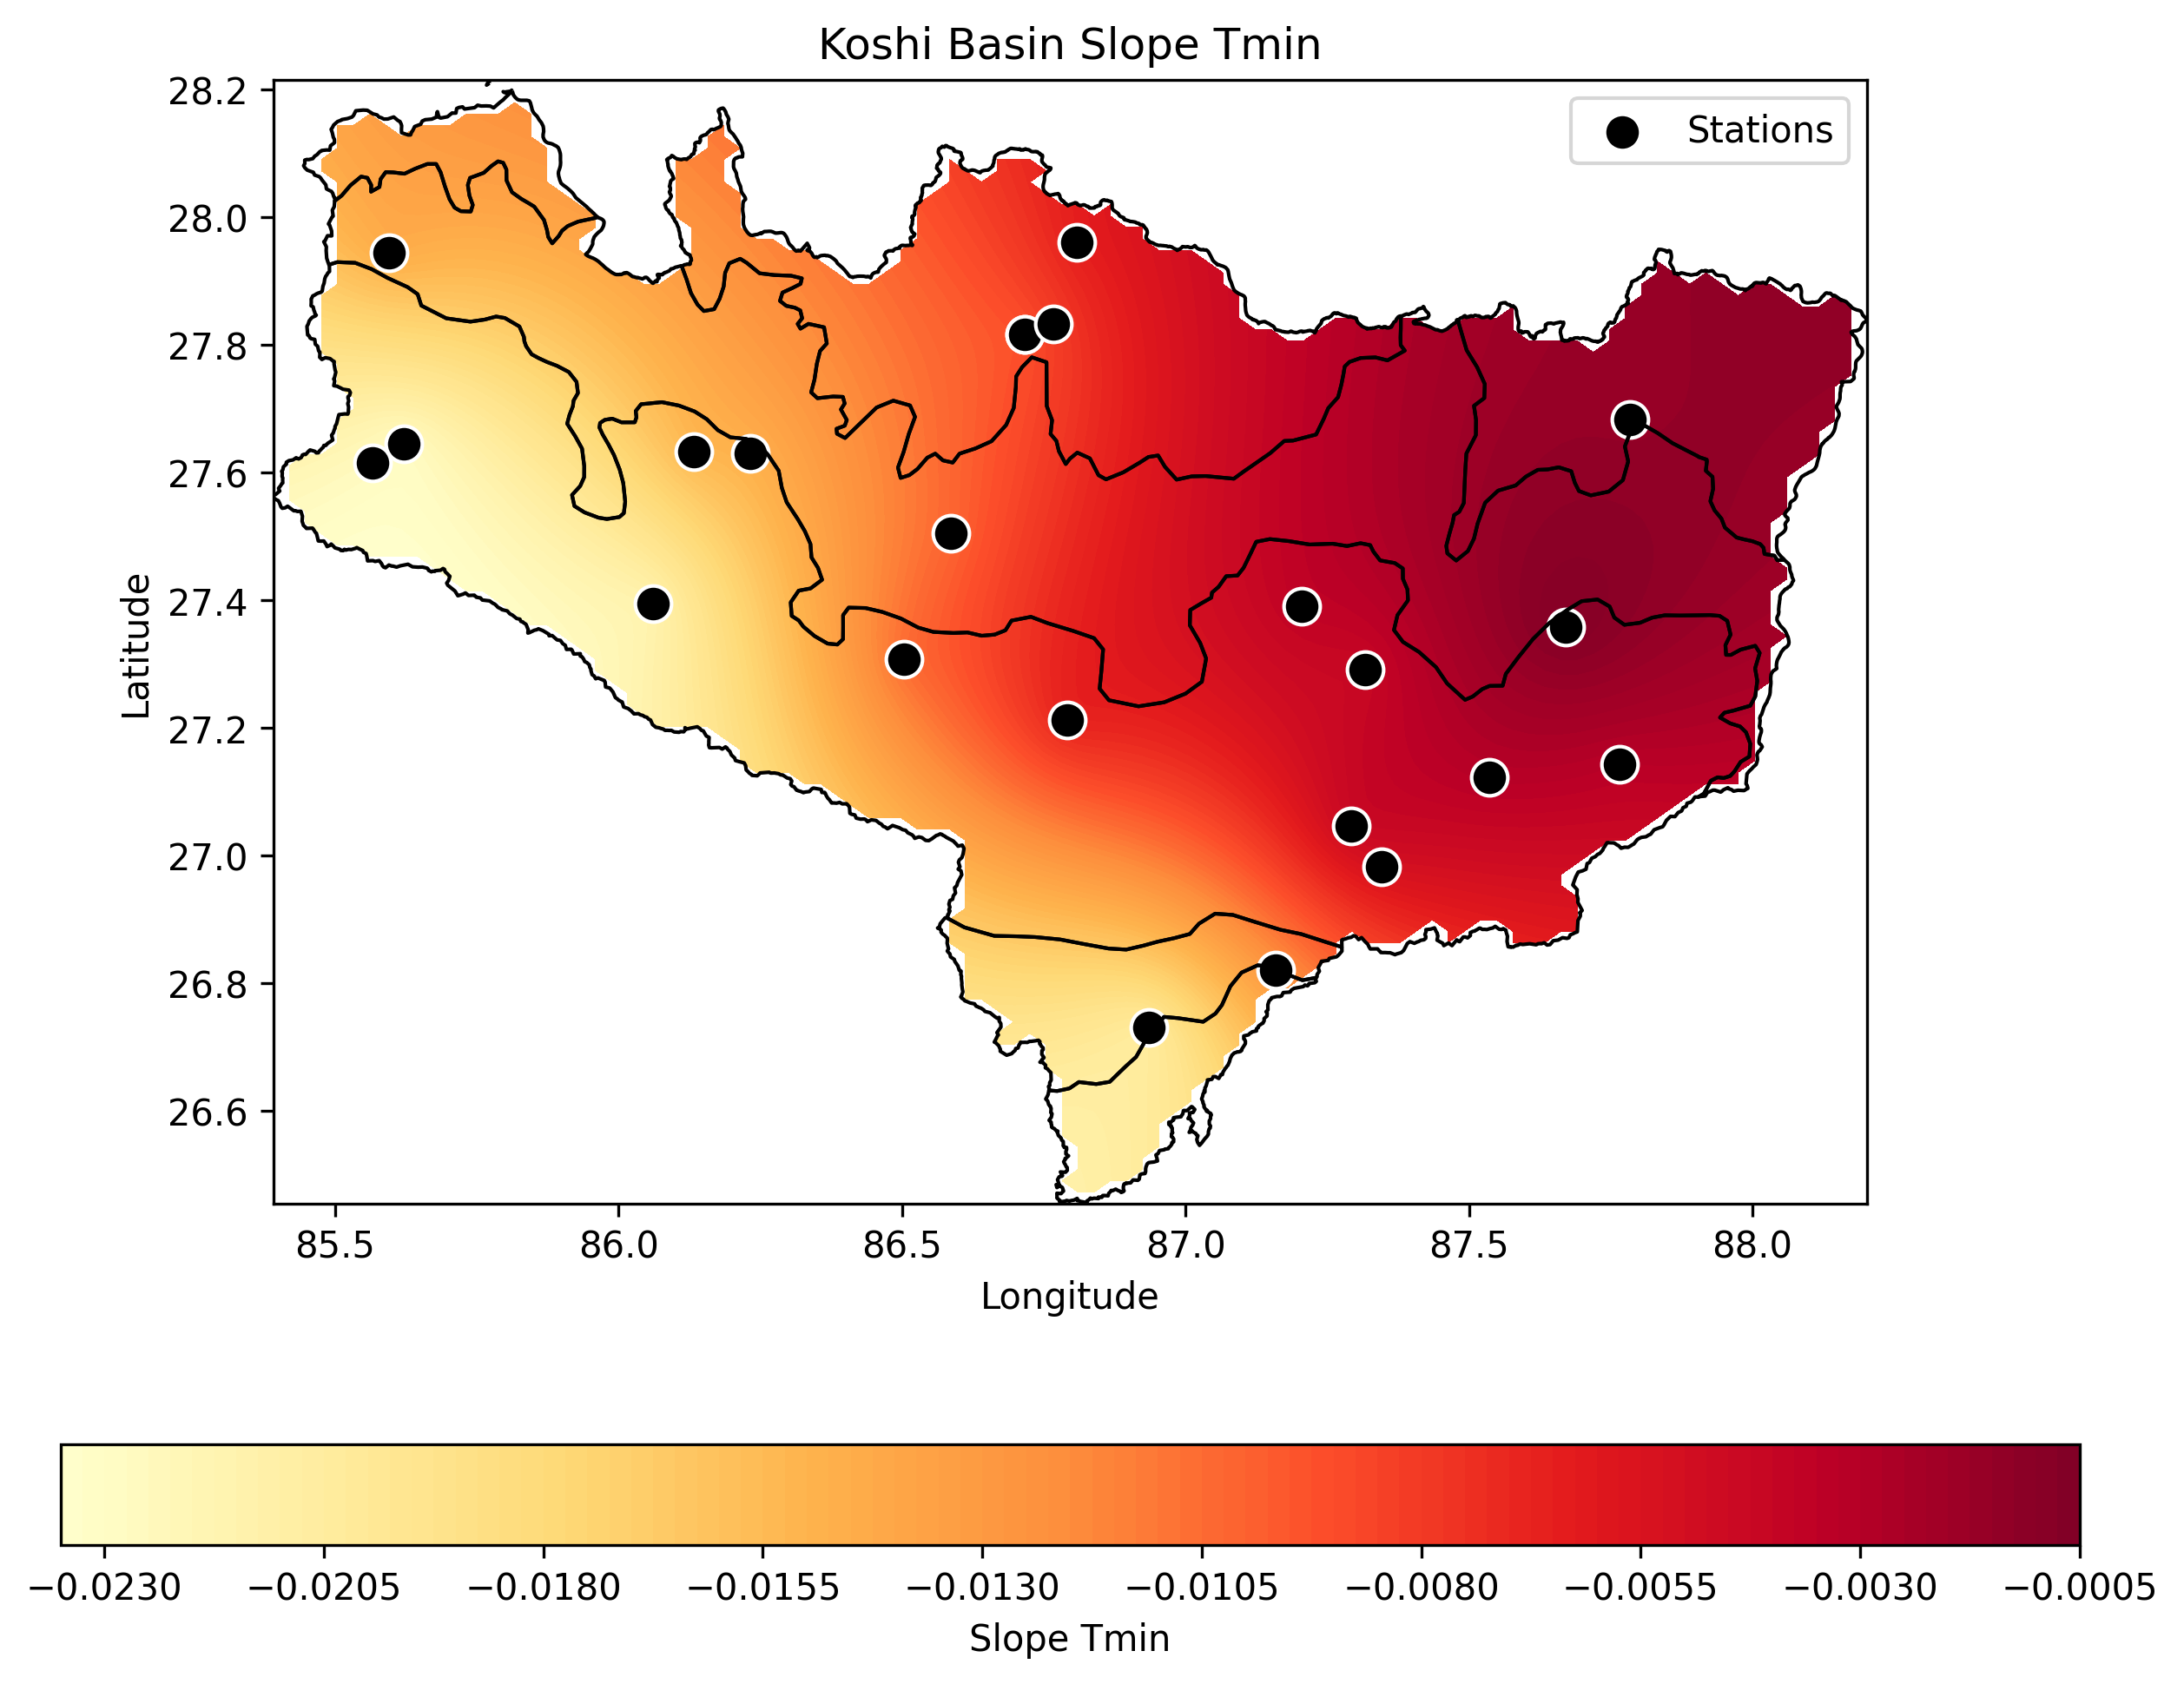
\includegraphics[width=\linewidth]{images/avg_krig_Koshi Basin Slope Tmin.png}
      \caption{Minimum Temperature Trend}
      \label{fig:basin_min_trend}
  \end{subfigure}
  \hfill
  \begin{subfigure}{0.45\textwidth}
      \centering
      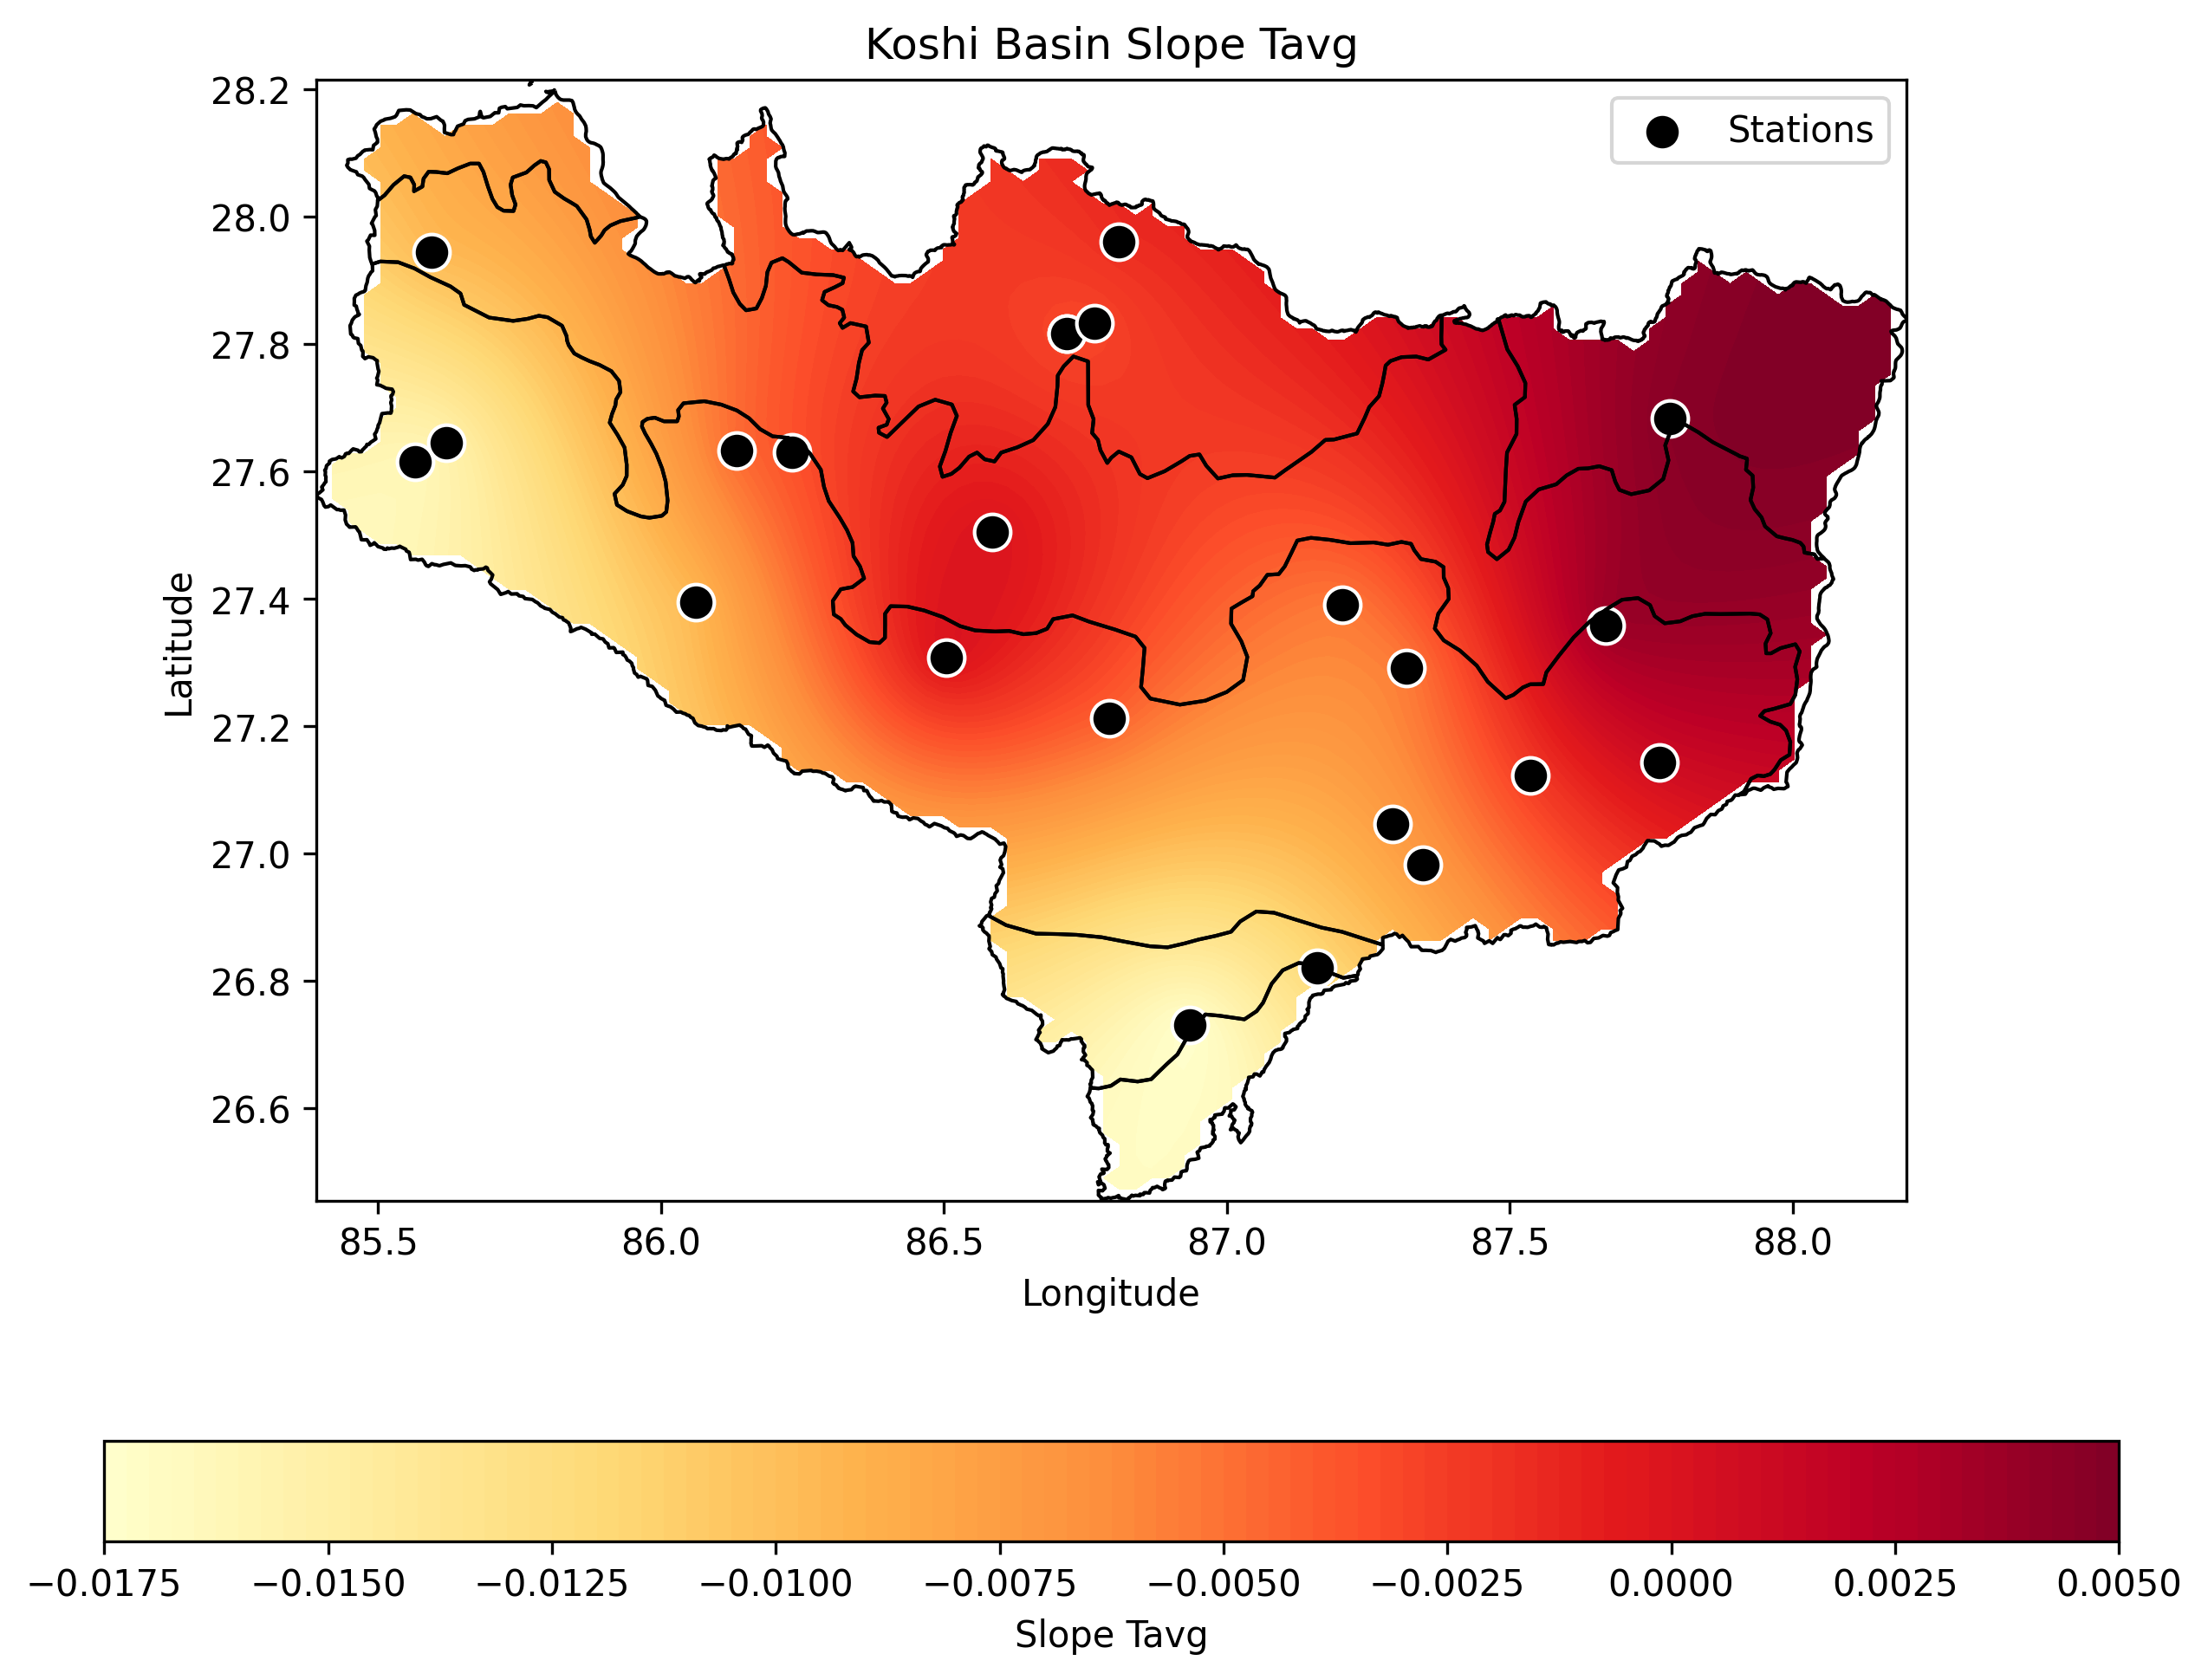
\includegraphics[width=\linewidth]{images/avg_krig_Koshi Basin Slope Tavg.png}
      \caption{Average Temperature Trend}
      \label{fig:basin_avg_trend}
  \end{subfigure}
  
  \vspace{0.5cm} % Adjust space between rows as needed
  
  \begin{subfigure}{0.45\textwidth}
      \centering
      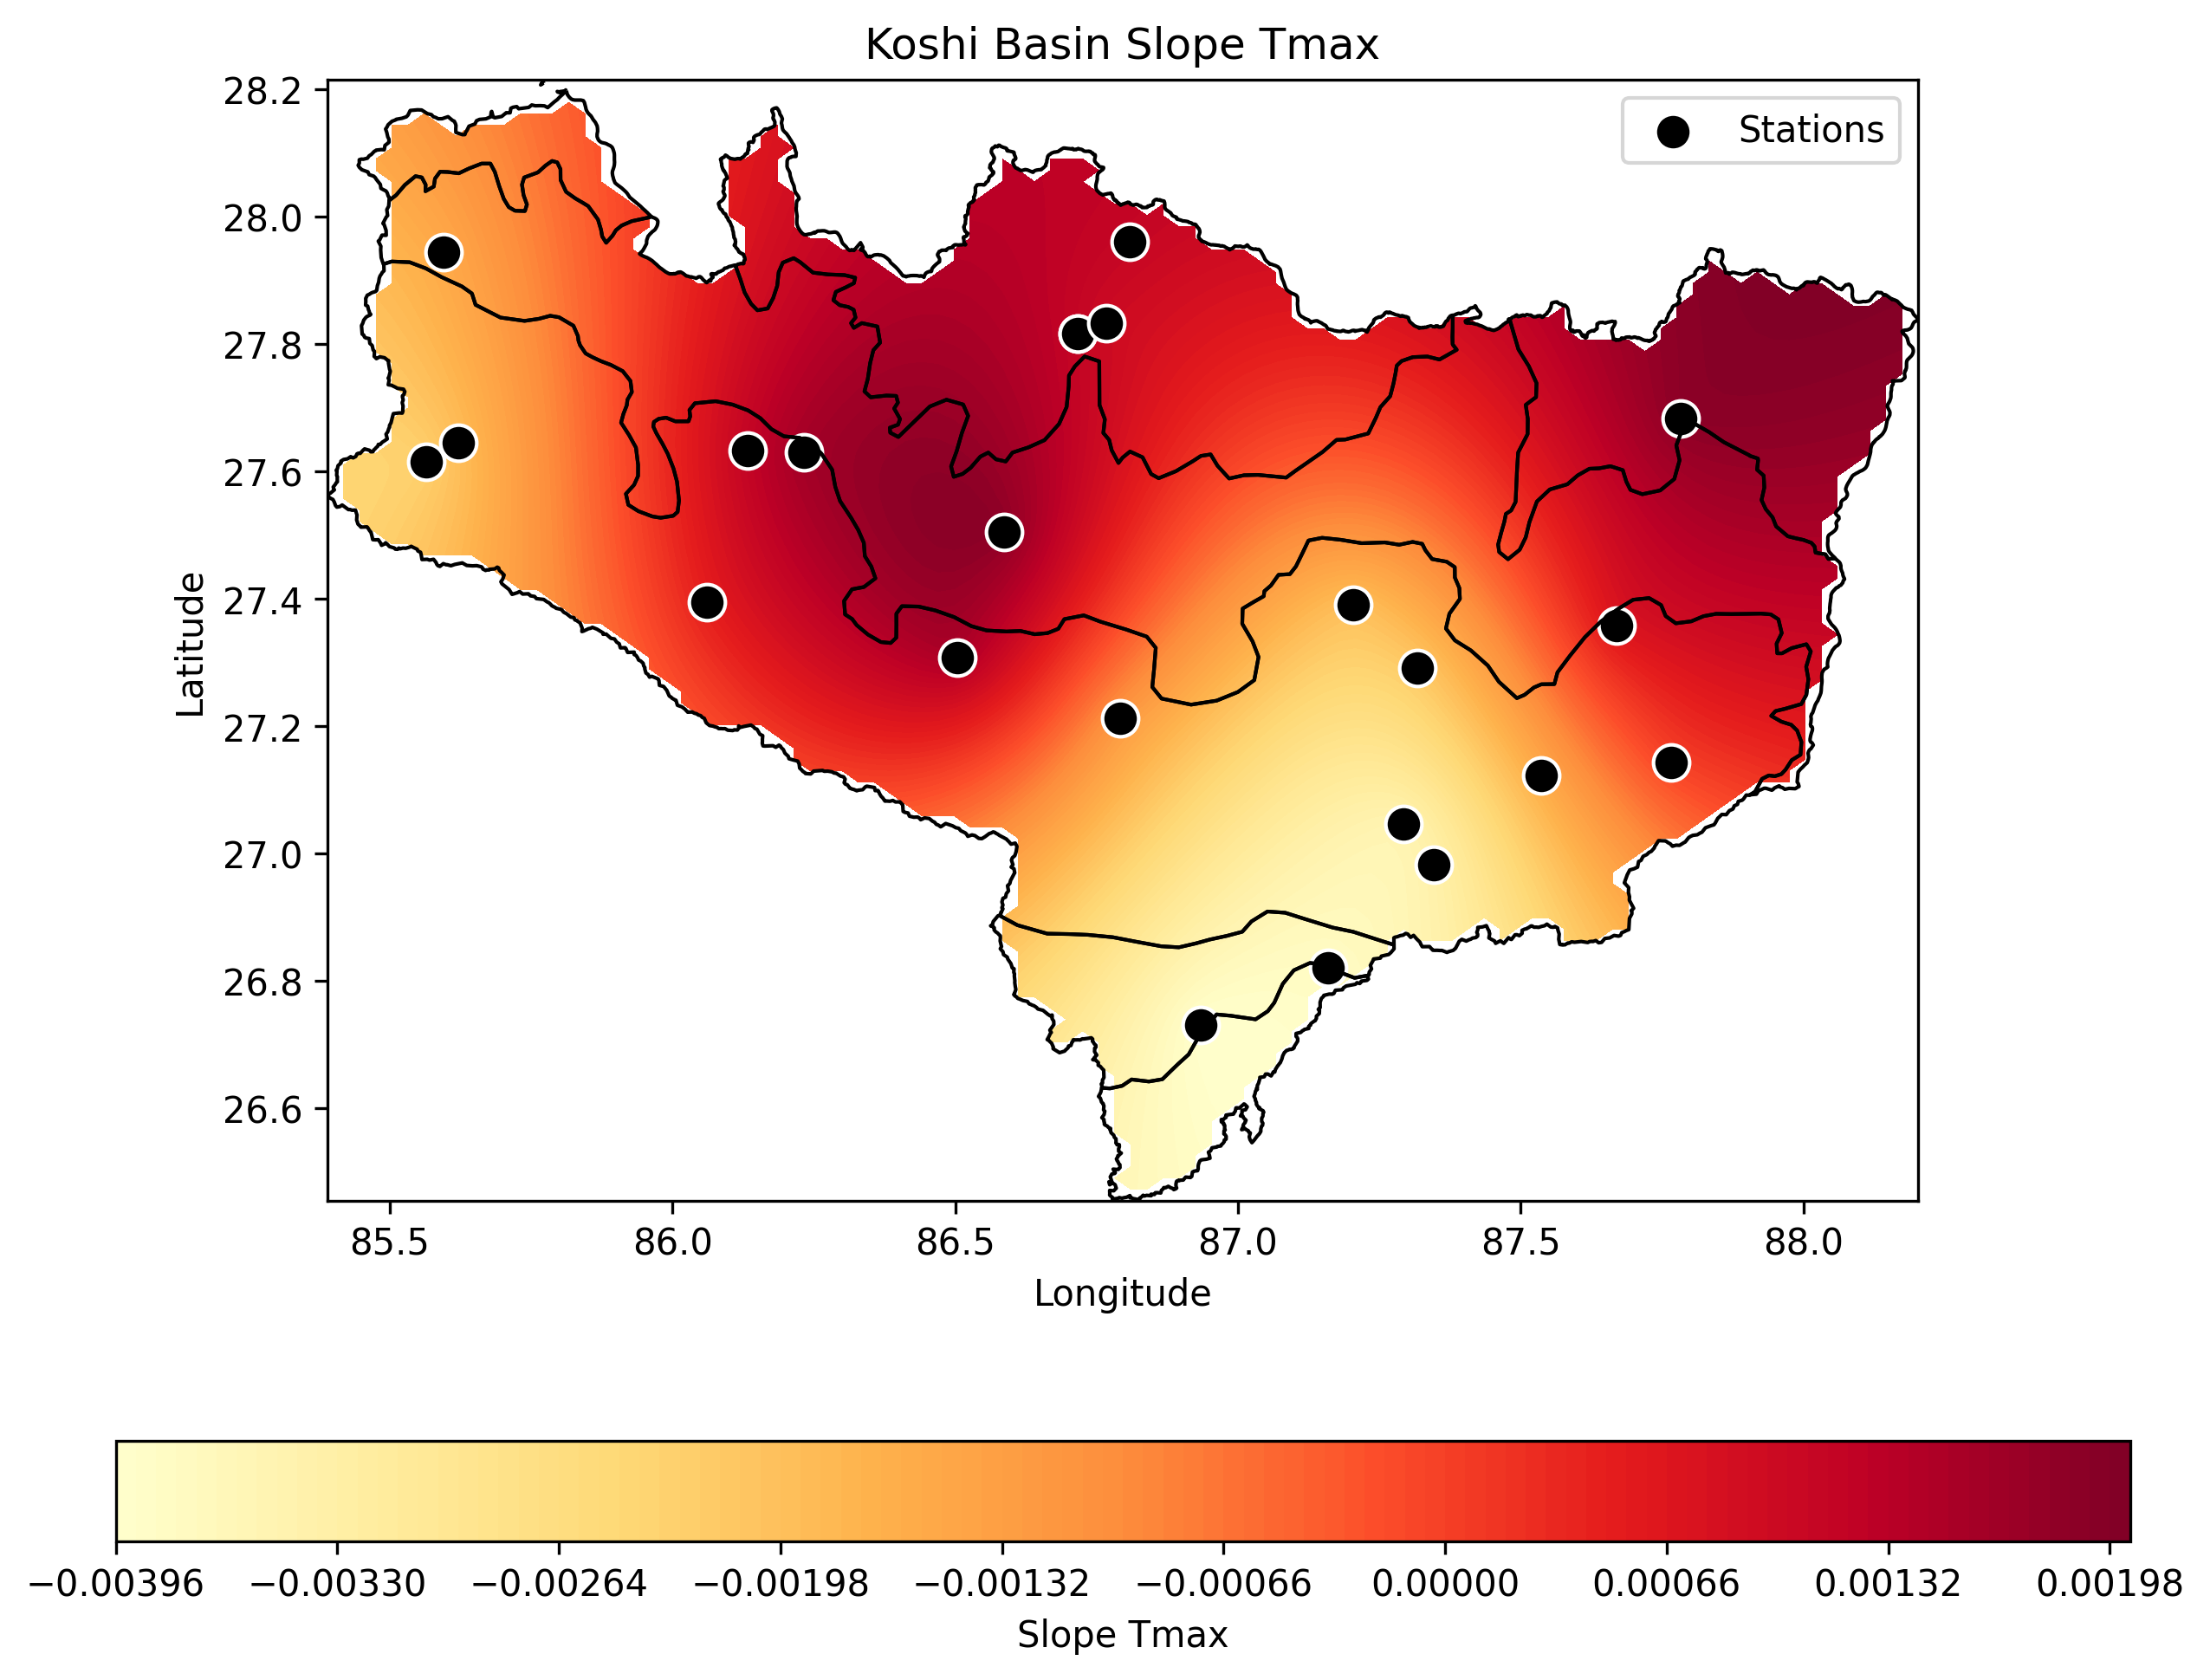
\includegraphics[width=\linewidth]{images/avg_krig_Koshi Basin Slope Tmax.png}
      \caption{Maximum Temperature Trend}
      \label{fig:basin_max_trend}
  \end{subfigure}
  
  \caption{Spatial distributions of annual temperature trends for the period 1962–2022 for (a) Tmin, (b) Tavg, (c) Tmax}
  \label{fig:krig_results}
\end{figure}

The results obtained from the analysis reveal a heterogeneous temperature trend across the Koshi basin region, as illustrated in Figure \ref{fig:krig_results}. An annual average of daily minimum temperatures shows an overall cooling trend, as shown in Figure \ref{fig:basin_min_trend}, ranging from -0.0005°C to -0.023°C, with higher elevations experiencing less cooling. As shown in Figure \ref{fig:basin_avg_trend}, the annual average temperatures reveal both warming and cooling trends, ranging from -0.0175°C to 0.005°C, where higher elevations tend to warm or cool less, when compared to the Tarai and Siwalik regions. Similarly, the annual average of daily maximum temperatures shows trends from cooling to slight warming (Figure \ref{fig:basin_max_trend}), ranging from -0.00396°C to 0.00198°C, with Tmax exhibiting a warming trend in higher elevation areas. Study conducted by Paudel et al. (2021) in transboundary Koshi basin for the years between 1980 and 2018, revealed an increase in the mean annual temperature by 0.084°C/ year in the mountain region (p = 0.0005), by 0.0975°C/year in the hill region (p = 0.0002), and by 0.0187°C/year in the Tarai region (p = 0.0206), with significant correlations throughout. 

\textcite{adhikari_x_2016} studied temperature trends from 1988 to 2010 in the Annapurna, Langtang, and Khumbu regions of Nepal. In the Khumbu region, moderate warming was observed across all seasons, with maximum temperatures rising by 0.0857°C/year in winter and 0.0628°C/year in pre-monsoon. The trend in the change of minimum temperatures was slightly different with a small increase of 0.0101°C/year in spring and a decrease of -0.0024°C/year during monsoon. Overall, mean temperatures increased by 0.0857°C/year in winter, with Khumbu showing lower trends compared to Langtang and Annapurna, particularly in minimum temperatures.

